\chapter{\red{Driving on the ground state manifold}}
\label{chap:groundStateManifoldDriving}
Of special importance in theory of the ground state manifold are geodesics. It is not yet clear what role they have in general, but there are a few known cases in which they play a particular role. As was mentioned in chapter \ref{chap:typesOfDriving}, one method to achieve low driving fidelity is \emph{path variation}. This means \emph{finding the best possible driving path}. One might say that the ground state manifold geodesics are a good candidate for this path, because they minimize the distance. The problem is that general fidelity driving does not happen on any state manifold and this premise cannot be used. The natural question is: "what types of drivings have minimal fidelity on geodesics?"


\subsubsection{Minimizing the distance on state manifolds}
Let's have a geodesic $\mathcal{G}(t)$ and some curve $\gamma(t)$ on the ground stat manifold, spanning between points $P_i,P_f\in \mathcal U$ during some time $T_f$, meaning
 $$\mathcal{G}(0)=\gamma(0)=P_i\in\mathcal U,\qquad \mathcal{G}(T_f)=\gamma(T_f)=P_f\in\mathcal U.$$

Excitation amplitude during infinitesimal quench is $\d s$, therefore $\sum_i \Delta s_i$ summed along path $\gamma(t)$ is the amplitude of transport along that path. This can be more rigorously expressed by functional
\begin{equation}
    s_\gamma=\int\limits_{\gamma(t)}\d s=\int\limits_{0}^{T_f}\sqrt{g_{\mu\nu}\dot\lambda^\mu\dot\lambda^\nu}\d t
\end{equation}
This is the entity, which is minimal if $\gamma$ is a geodesic. Before moving on, lets quickly review the proof of this statement.

\begin{proof}[proof: Geodesics minimize the distance on manifold]
    Functional of distance is
    \begin{equation}
        s=\int\limits_0^{T_f} \sqrt{g_{\mu\nu}\d\lambda^\mu\d\lambda^\nu}=\int\limits_0^{T_f} \sqrt{g_{\mu\nu}\der{\lambda^\mu}{t}\der{\lambda^\nu}{t}}\d t \eqqcolon \int\limits_0^{T_f} \mathcal{L}(t,\lambda^\mu,\dot\lambda^\mu)\d t
    \end{equation}
    for 
    \begin{equation}
        \mathcal{L}=\sqrt{g_{\mu\nu}\dot\lambda^\mu\dot\lambda^\nu}.
    \end{equation}
    Using Euler-Lagrange equations 
    \begin{equation}
        \der{\mathcal{L}}{\lambda^\mu}-\der{}{t}\der{\mathcal{L}}{\dot\lambda^\mu}=0,
    \end{equation}
    we get for $g_{\mu\nu}=g_{\mu\nu}(\lambda^\mu)$ second order differential equation
    \begin{equation}
        \ddot\lambda^\mu+\Gamma^\mu_{\;\;\alpha\beta}\dot\lambda^\alpha\dot\lambda^\beta=0\qquad \Gamma^\mu_{\;\;\alpha\beta}=\frac{1}{2}g^{\mu\kappa}\left(g_{\kappa\alpha,\beta}+g_{\kappa\beta,\alpha}-g_{\beta\alpha,\kappa}\right),
        \label{eq:geodesicEquaiton}
    \end{equation}
    which is the Geodesic equation.
\end{proof}




% \textcolor{blue}{Polkovnikov for some special case: They play a role of "maximum fidelity at any time" transport, meaning at any given time $t$ the fidelity on corresponding point on geodesics will be less than of $\gamma$
% $$F(\mathcal{G}(t))<F(\gamma(t)).$$ }







\section{Minimizing the energy variance}
The driving can be restricted to the ground state manifold only in approximation, such that the excited parts of wave-function can be neglected in every step. From \cite{Bukov2019}, we have the following theorem.

\begin{thm}
    \label{thm:polkovnikov}
    For any fast-forward Hamiltonian\footnote{The system is driven to the target state in some fixed time.} $\HH(\lambda(t))$ driven along one dimensional path $\lambda: \R\mapsto \R$ using time $t$ as parametrization, there exist driving speed, for which the fidelity is close to one, $F(t)\approx 1 \;\forall t\in[0,T_f]$, and the energy fluctuations $\delta E^2$, averaged along the path, are larger than the geodesic length $l_\lambda$
    \begin{equation}
        \int\limits_0^T\sqrt{\delta E^2(t)}\d t \eqqcolon l_t\geq l_\lambda \coloneqq \int\limits_{\lambda_i}^{\lambda_f} \sqrt{g_{\lambda\lambda}\d \lambda\d \lambda} =\int_0^T \sqrt{g_{\lambda\lambda}}\frac{\d \lambda}{\d t}\d t.
    \end{equation}
    The length $l_\llambda$ is defined in parametric space (with metric tensor $g_{\lambda\lambda}$) and is generally larger than the distance between wave functions, so called \emph{the absolute geodesic}, defined with $G_{\mu\nu}$. From its definition, we can see that it corresponds to the metric tensor as we use it.
    
    
    
    The energy variance is 
    \begin{equation}
        \delta E^2\coloneqq \braket{o(t)|\HH(t)^2|o(t)}-\braket{o(t)|\HH(t)|o(t)}^2=\braket{\partial_t (t)|\partial_t o(t)})_c=G_{tt},
    \end{equation}    
    where in second step the Schr\"odinger equation was used. The Metric tensor in parametric space is defined as
    \begin{equation}
        g_{\lambda\lambda}\coloneqq \braket{\partial_\lambda o(t)|\partial_\lambda o(t)})_c
    \end{equation}
\end{thm}


\begin{proof}
    \begin{equation}
        \delta E^2\equiv \braket{o(t)|\HH(t)^2|o(t)}_c=\dot\lambda^2 G_{\lambda\lambda}+\O(\dot\lambda^4),
    \end{equation}
    where $\O(\dot\lambda^4)$ needs to be positive for any real-valued Hamiltonian. This comes from the fact, that it has instantaneous time-reversal symmetry.
\end{proof}

The conjecture can be extended to an arbitrary dimensional path. The main problem of this conjecture is the statement \emph{close unit fidelity protocol}. It is not clear how good the approximation need to be. This makes the statement much weaker, because it says: \emph{For any driving, there exist driving speed for which the energy variance will be minimized on geodesics.}









\section{Transport using quenches}
\label{sec:quenches}
Unifying the ground states $\ket{o(\llambda)}$ over all points $\llambda\in\mathcal U$ in the parameter space, we get the ground state manifold. Here the fidelity $f$ and distance $s$ are defined
\begin{equation}
    \d s^2 = 1-F = 1-\left|\braket{o(\bm\llambda+\delta\bm\llambda)|o(\bm\llambda)}\right|^2.
    \label{eq:distanceOnM0_1}
\end{equation}

The final fidelity of transport on $\M$ is then
\begin{equation}
    F=\iint\limits_{\gamma(t)} g_{\mu\nu}\d\lambda^\mu\d\lambda^\nu = \int_{t_i}^{t_f}\underbrace{\int_{t_i}^\tau g_{\mu\nu}\der{\lambda^\mu}{t}\der{\lambda^\nu}{t} \d t}_{\mathcal{L}(\lambda^\mu,\dot\lambda^\mu,\tau)}\d \tau .
\end{equation}
Using Euler-Lagrange equations for time-independent $g_{\mu\nu}=g_{\mu\nu}(\lambda^\mu)$, leads to
\begin{equation}
    \int_{t_i}^{\tau}\left[g_{\mu\nu,\kappa}\dot\lambda^\mu\dot\lambda^\nu - \der{}{t}\left[g_{\mu\nu}\left(\delta^\mu_\kappa\dot\lambda^\nu+\dot\lambda^\mu\delta^\nu_\kappa\right)\right]\right]\d t=0,
\end{equation}
which needs to be zero for integration over any subset $(t_i,\tau)$. This can be achieved for any path only if the integrand itself is zero, which happens if the geodesic equation is satisfied.

The fidelity $F$ measures transition probability between two eigenstates, $\ket{\psi_1}$, $\ket{\psi_2}$, of two different Hamiltonians (in our case, of one Hamiltonian with two different values of driving parameter $\llambda_1$, $\llambda_2$). Those two states belong to the same Fiber space $\PH(\llambda)\times \mathcal U$ from which the coefficients $(\text{index of energy state}; \llambda)\in (\Z,\R^n)$ are taken. Because $\PH(\llambda)$ are canonically isomorphic for $\forall \llambda\in \mathcal U$, there is no problem in parallel transport from one space to another, which is needed for evaluating the braket $\braket{\psi(\llambda_1)|\psi(\llambda_2)}$. This is important notice, because the integration in braket can be performed only if both elements belong to the same space.

The distance minimization runs into some interpretation problems. On one hand, minimization of the distance is equivalent to maximization of the sum of infinitezimal fidelities along the path (we say we \emph{maximize the fidelity along the path}). On the other hand we are using only ground states in every step of the transport, therefore defining the fidelity to be one. There are actually two ways out of this confusion. \emph{Perturbed adiabatic driving} and \emph{Transport using quenches}.


\subsubsection{Closed adiabatic driving}
It the first case, we imagine at every point of transport, that the fidelity is small enough, that for some small parameters $\delta_i\in \mathbb{C}$, we can write the transport over distance $\d s$ in eigenbasis at time $t=0$, as
$$\ket{o(\llambda_i)}\equiv \begin{pmatrix}
    Z_0(\llambda_i)\\
    0\\
    \vdots \\
    0
\end{pmatrix} \overset{\text{transport }\d s}{\longrightarrow} \ket{o(\llambda_i+\delta \llambda)}\equiv\begin{pmatrix}
    Z_0(\llambda_i+\delta \llambda)\\
    0\\
    \vdots \\
    0
\end{pmatrix} +\underbrace{\begin{pmatrix}
    0\\
    \delta_1(\llambda_i+\delta \llambda)\\
    \vdots \\
    \delta_n(\llambda_i+\delta \llambda)
\end{pmatrix}}_{\mathbf{\Delta}(\llambda_i+\delta \llambda)}, $$
where the last term is neglected, because
$$\braket{\Delta(\llambda)|o(\llambda+\delta\llambda)}\approx 0.$$

This might have interesting implication for slow transports, or small distance transports. For slow transports, this condition is hardly fulfilled, because one needs to neglect the sum of many of these terms. For example when some slow thermalization is considered during transport. The easier way would be to reset the state into the ground-state, when the fidelity gets too far from 1. This can be achieved by projecting the state $\ket{\psi(t)}$ to the ground state $\ket{0(t)}$ periodically, such that every time the fidelity is almost one. These small jumps are sometimes called \emph{quenches}. Let's see the mathematics behind this idea.




If we imagine $\delta\llambda$ to be finite (not infinitely small, as the notation suggests), the \emph{transport} means \emph{doing a sequence of quenches and measuring the system after every quench}. This leads to the \emph{quantum Zeno effect}. In this case it can be shown directly by splitting the distance $s$ on parametric space $\mathcal U$ to $N$ equal pieces. The fidelity for $N$ splits will then be
\begin{equation}
    F(N)=(1-\Delta s)^N=\left(1-\left(\frac{s}{N}\right)^2\right)^N \;\;\overset{N\rightarrow\infty}{\longrightarrow}\;\; 1,
\end{equation}
meaning the consequent measurements on the system leads to collapse to the instantaneous eigenstate and the adiabatic condition for transport holds ($F=1$). 

Such measurements can be achieved by fast thermalization of the system. If the finite speed thermalization with $N=T/\tau$ for the mean time between two measurements $\tau$, we get
\begin{equation}
    \begin{split}
        \log f(N) &= N \log \left(1-\left(\frac{s}{N}\right)^2\right) = -\frac{s^2}{N}+o\left(\frac{s^4}{n^3}\right)\\
        f(N) &= \exp\left(-s^2\frac{\tau}{T}-\frac{s^4}{2 N^3}\dots\right) = \exp\left(-s^2\frac{\tau}{T}\right)\left(1+o\left(\frac{s^4}{N^3}\right)\right)
    \end{split}
\end{equation}

Some notion of the space of our Hamiltonian can be seen by quenching from $(\lambda_i;\chi_i)=(0;0)$ to $(\lambda;\chi)$ in Figure \ref{fig:quenchFidelityFrom00}.


In Figure \ref{fig:plotsFidelityQuenches}, we can see equidistant points, meaning $\int_{a}^{b} \d s=\text{const}$ between every two neighboring points on ground state manifold geodesics. One can see that if the system is measured periodically, the quenches jump smaller distances when closer to a point of degeneracy. Decreasing time step $\Delta t$ has no effect on the relative fidelity of quenches during the evolution but has an effect on their absolute fidelity. As one would expect from quantum Zeno effect, when $\Delta t\rightarrow 0$, the transport becomes adiabatic, and the fidelity at any time will become $1$. See that the shape of the curves looks similar in the columns, but their magnitude decreases.

\begin{figure}[H]
    \centering
    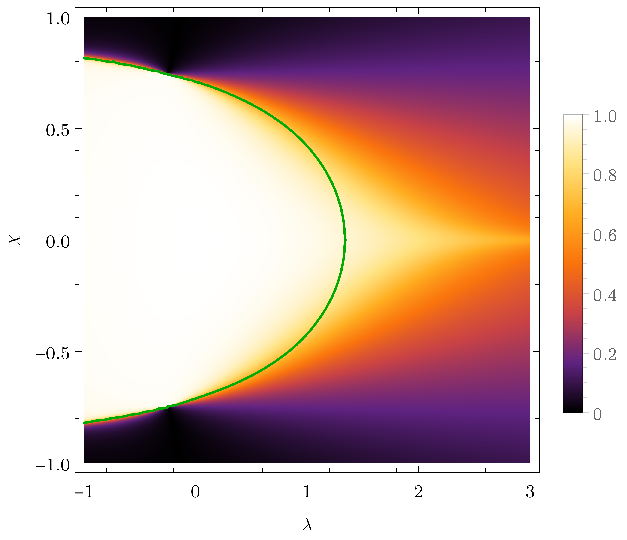
\includegraphics[scale=1.2]{../img/quenchFidelityFrom00.pdf}
    \caption{Arctangens of the fidelity of quench from $(\lambda_i;\chi_i)=(0;0)$ to the coordinate $(\lambda;\chi)$.}
    \label{fig:quenchFidelityFrom00}    
\end{figure}

% \begin{figure}[H]
%     \centering
%     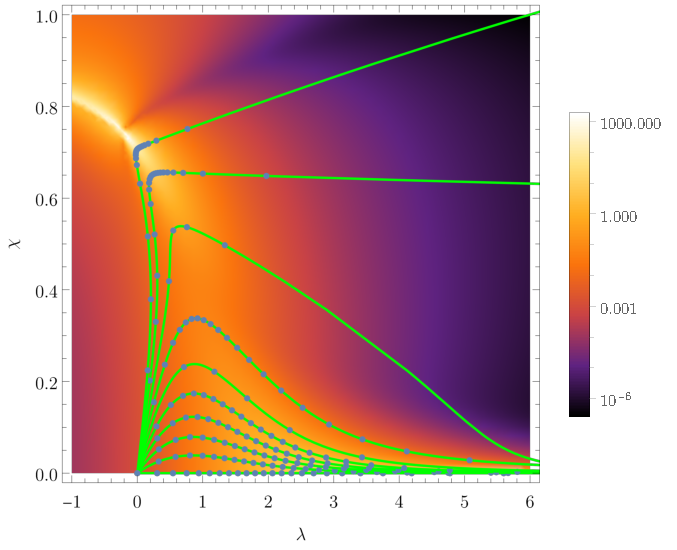
\includegraphics[scale=1.2]{../img/equidistantPointsOnPath.pdf}
%     \caption{Equidistant points on geodesics of the ground state manifold.}
%     \label{fig:equidistantPointsOnPath}    
% \end{figure}

\begin{figure}[H]
    \centering
    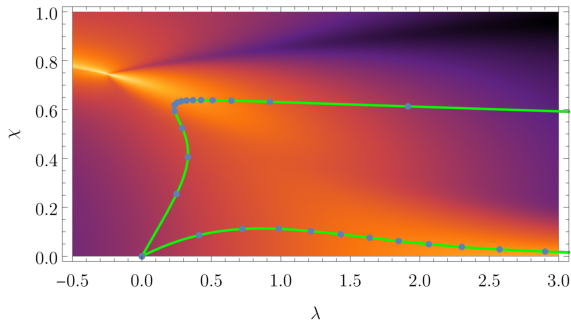
\includegraphics[scale=1.2]{../img/bg123.pdf}
    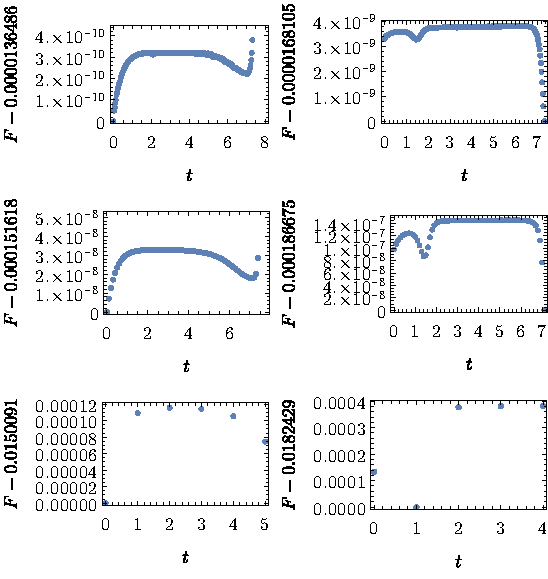
\includegraphics[scale=0.6]{../img/plotsFidelityQuenches.pdf}
    \caption{Fidelity for sequential quenches along geodesics (see green lines on top). Left (right) column corresponds to lower (upper) geodesic. Time steps from top are $\Delta t\in \{0.03,0.1,0.5\}$. Time difference between points in the plot on top is $\Delta t=0.5$.}
    \label{fig:plotsFidelityQuenches}    
\end{figure}


